\ifdefined\included
\else
\setcounter{chapter}{2} %% Numéro du chapitre précédent ;)
\dominitoc
\faketableofcontents
\fi

\chapter{Ontologenius: A semantic memory for HRI}
\chaptermark{Ontologenius}
\label{chap:ontologenius}
\minitoc
\label{chap:2}

In this chapter, we present the software Ontologenius. It is a lightweight and open-source software to store an ontology, perform reasoning on it, update it, and query it. Ontologenius has been developed especially for \acrlong{hri} application. In this way, it is able to manage several ontology instances in parallel and puts a focus on the concepts' names in natural language. It aims to be used as a server, shared by an entire robotic architecture, providing consistent and always up to date knowledge to every components of the architecture. Consequently, it is thread-safe and can be queried by several components at a time while being constantly updated.

A previous version of this contribution has been presented and published at the RO-MAN 2019 conference~\cite{sarthou_2019_ontologenius}. Due to the evolution of the software since this publication, the current chapter presents new features and a more mature contribution.

\section{Design and features}

In this section, we first explain our choice to use ontology as a means of representing knowledge, both from the point of view of its expressiveness and its growing use in robotics. Then, we present the wanted features and the level of expressiveness we have selected for this software. Finally, we draw a formalism of the kind of ontology we will use all along this thesis.

\subsection{Why an ontology?}

In cognitive psychology, we saw that semantic memory refers to the encyclopedic knowledge of words associated with their meanings. After several studies about participants response times to questions, some authors have proposed a model of this semantic memory as being a semantic network~\cite{collins_1969_retrieval, collins_1970_does}. With this model, they put the hypothesis that knowledge is organized in a hierarchic way, respecting a principle of inclusion among classes. For example, a class representing the concept of cat would inherit an upper class, representing the concept of animal. In addition, instances of these classes would be linked to others through properties, and in the same way, as for the classes, a notion of hierarchy over the properties would exist. Such a structure of knowledge in humans would allow a cognitive economy as well as efficient storage of this knowledge. Even if they were not the first to formalize the principle of a semantic network, Collins and Quillian have provided prominent works and computer implementations.

As reported in~\cite{prasad_2020_knowledge}, such a semantic network, also called semantic graph or knowledge graph, is today frequently used as knowledge representation in robotic applications to represent among others:

\begin{itemize}
  \item the categories of entities at different levels of abstraction~\cite{balint_2018_variations}, e.g. a handle is a physical object
  \item the characteristics of entities~\cite{tenorth_2017_representations}, e.g. a fridge has a handle
  \item the function or purpose of entities~\cite{paulius_2019_functional}, e.g. the fridge handle allows to open the fridge
  \item the location of an entity regarding another one (i.e. spatial relations)~\cite{singh_2020_fuzzy}, e.g. the milk bottle is in the fridge
\end{itemize}

This is on the basis of this knowledge that we can then create programs to provide cognitive capabilities to robots. Here is an important point, this knowledge should support the components of the architecture but is not necessarily part of it. It is called the knowledge-enabled robot programming paradigm~\cite{beetz_2012_cognition}, where the knowledge is separated from the program. It allows to have several subsystems of a same robotic architecture, each providing a specific cognitive capability but all sharing the same knowledge. The choice to share common knowledge leads to important challenges requiring first to agree on the knowledge content and second to provide it in a machine-understandable way. Considering the use of a semantic network as knowledge representation, the use of ontology has tended to respond to these challenges.

The first definition of an ontology has been proposed by Guber in~\cite{guber_1993_translational} as: \textit{``an ontology is an explicit specification of a conceptualization''}. Later, Borst~\cite{borst_1999_construction}, has introduced two new concepts defining an ontology as a \textit{``formal specification of a shared conceptualization''}. The new concepts are the notions of ``formal'' and ``shared''. Merging these two definitions, Studer et al.~\cite{studer_1998_knowledge} reached the definition: \textit{``An ontology is a formal, explicit specification of a shared conceptualization''}. With this last definition, we start to see that an ontology can be a powerful tool to create a \acrfull{kb} common to an entire robotic architecture and used by subsystems providing specific cognitive capabilities.

Even if all the previous definitions trend to refine what is an ontology, they all rely on the common notion of conceptualization for which no formal definition is provided. A former definition, presented in~\cite{genesereth_1987_logical}, was:

\begin{quote} 
\centering 
\textit{
``A body of formally represented knowledge is based on a conceptualization: the objects, concepts, and other entities that are assumed to exist in some area of interest and the relationships that hold among them. A conceptualization is an abstract, simplified view of the world that we wish to represent for some purpose. Every knowledge base, knowledge-based system, or knowledge-level agent is committed to some conceptualization, explicitly or implicitly.''}
\end{quote}

However, as explained by Guarino in~\cite{guarino_2009_ontology}, such a definition of a conceptualization does not correspond to our intuition either our need for an ontology. Indeed, we do not want the conceptualization to depend on the current situation. It should rather be what is common to any situation, allowing to represent them in a uniform way. As explained in~\cite{guarino_1995_towards}, when the world is modified, the conceptualization should stay the same. We are thus interested in the meaning of the concepts used to describe a world state. However, the final definition of a conceptualization provided by Guarino goes with difficulty in this direction despite its initial goal. For the simplicity of the current purpose, the conceptualization should be the meaning of any concept allowing to represent a given situation or world state. Consequently, an ontology could be defined as:

\begin{quote} 
\centering 
\textit{a formal and explicit specification of the shared meaning of any concept allowing to represent a given situation.}
\end{quote}

In other words, an ontology aims at constraining the interpretation of a used vocabulary. It is thus a logical theory. However, looking at the literature, we notice that the definition of an ontology is still today blurry. Indeed, even if it represents the meaning of the usable concepts, we want to apply it to the \acrshort{kb} representing a given world state, even if it evolves. Where a semantic network would represent this instantiation, because the meaning of its edges could be defined by the use of an ontology, in this thesis, we will use the term ontology to refer to \textbf{a semantic network owning a restriction on the interpretation of the used vocabulary}. As the goal of this thesis is not to model these restriction rules but rather to use them, it should not lead to any confusion.

Considering the study of ontology in robotic, and more generally in computer science, we can distinguish three kinds of contribution:

\begin{itemize}
  \item ontology creation,
  \item ontology storage and inference,
  \item framework using ontology
\end{itemize}

Ontology creation focuses on the definition of vocabulary and rules. The created ontologies are often divided into four categories: upper-level, reference, domain, and application. The upper-level ontologies define widely applicable concepts, transversal to several disciplines. The more used are DOLCE (Descriptive Ontology for Linguistic and Cognitive Engineering) \cite{masolo_2003_dolce}, Cyc \cite{lenat_1989_building}, or SUMO (Suggested Upper Merged Ontology) ~\cite{niles_2001_towards}. Reference ontologies are based on upper-ontology and describe the vocabulary of a discipline, like engineering or medical. For example, \cite{schlenoff_2015_ieee} covers robotics and automation. Domain ontologies aim at refining a discipline, focussing on a more restricted domain in it, like the SOMA ontology~\cite{bessler_2020_foundations} focussing on activities representation. Finally, applications ontologies extend domain ontologies for precise applications. The ontology design uses languages like RDF (Resources Description Framework), FOL (First Order Logic), or OWL (Web Ontology Language). Each language comes with characteristics like formality or computability.

Using these ontologies, numbers of frameworks have been developed to support high-level reasoning process in robotic applications. Among them, we find ontology used for decision making, situation assessment, planning, or belief maintenance. A complete review of these reasoning capabilities and the corresponding frameworks is available in~\cite{olivares_2019_review}. Among the reviewed frameworks, the emblematic ones are KnowRob~\cite{tenorth_2013_knowrob}, ROSETTA~\cite{stenmark_2013_knowledge}, CARESSES~\cite{bruno_2017_caresses}, RoboBrain~\cite{saxena_2014_robobrain}, or ORO~\cite{lemaignan_2010_oro}.

The last contribution type, being the one of the current chapter, is the ontology storage and inference to form a \acrlong{kb} on which the framework can rely to perform high-level reasoning. KnowRob uses Prolog~\cite{wielemaker_2003_prolog} with a library to manage RDF triples. ROSETTA uses a Sesame triple store~\cite{broekstra_2002_sesame}. ORO uses the Jena triple store in addition to the Pellet~\cite{sirin_2007_pellet} reasoner. Finally, RoboBrain uses a custom graph database. We can see that no standard solution has emerged as it mostly depends on the application needs in terms of query capability, expressiveness support, or technical support and compatibility. As other tools we can find in C++ owlcpp~\cite{levin_2011_owl} based on Raptor and Fact++~\cite{tsarkov_2006_fact}, or in Python RDFlib, OWLReady2, or AllegroGraph.

To sum up, a \acrlong{kb} in the form of an ontology, can be viewed as a semantic graph relying on a formal and explicit specification of the shared meaning of concepts used to represent a given situation. In order to be used in a framework to perform high-level reasoning, ontology has to be stored to expose the knowledge it contains to other components. No standard storage solution has emerged so far as it mostly depends on the application needs. Consequently, in the next part of this section, we discuss our needs with a focus on \acrlong{hri} applications and taking inspiration on the existing solutions, we define the features we want for our storage system.

%This initial model has since been formalized as an ontology \cite{berners-lee_semantic_2001} and is already widely used in the semantic web.

\subsection{Desired features}

\paragraph{Work as a server:} The robotic architecture we target is composed of several modules, able to communicate. On the top of the architecture, we consider a supervision system, being a kind of ``puppet-master'' which call each component when needed. A common issue with such an architecture is that each component owns a part of the general knowledge which can lead to inconsistencies. Consequently, the \acrlong{kb} we want should be a server, accessible by query and update by any component. It thus provide uniform knowledge among the architecture. To create a server, we could use any existing tool and attach a communication layer to it. This is for example the case of ORO, which work as a sever, based on the Jena triple store and providing a Telnet interface to send the queries and updates.

\paragraph{Support multiple instances:} Since we target \acrshort{hri} application, we need to be able to represent an estimation of the others knowledge. Where some could use a single \acrlong{kb} to represent the robot knowledge as well as the humans' knowledge, we want our software to support the ``self-other distinction''. It is presented in~\cite{pacherie_2012_phenomenology} as the fact that ``for shared representations (...) to foster coordination rather than create confusion, it is important the agents be able to keep apart representations of their own and other's actions and intentions''. To the best of our knowledge, ORO is the only software proposing this ability. However, it uses a simple way to implement it by running several instances of the same triple store, each attached to an agent. As we will see during this chapter, in robotic application such a solution is not sufficient. For task planning usage, we could need to estimate a future state of a \acrshort{kb}. To implement this feature, we need to be able to capture the state of a \acrshort{kb} at a given instance then be able to modify it without impacting the original \acrshort{kb}. At the date of this thesis, no tool provides this possibility.

\paragraph{Query at the semantic level:} As explained in~\cite{broekstra_2002_sesame}, to query RDF graphs, three levels are possible. Considering an ontology written in XML, the syntactic level would query the XML structure. Consequently, it would query a tree rather than a graph. A query would be ``give me the resources nested in a \textit{Description} element having the attribute \textit{about} with the value X''. It is thus dependant on the language and requires to known the used keywords. The structural level, as available in~\cite{lassila_1998_resource}, provides an abstraction to the language. It allows query of the kind ``give me all the elements of type A'' regardless of how it is represented in the language. However, the structural only looks at the explicit triples. If B is a subtype of A and the element x is described as being of type B, requesting for the elements of type A, x will not be returned. The last query level is the semantic level which is not limited to explicit knowledge. At this level, requesting for the elements of type A, x would be returned as x is of type B and B is a specification of A. This means that we do not consider a simple triple store trying to match patterns. To support this query level, two solutions can be used: computing the closure of the graph (adding A as a type of x and storing it), or inferring it at query. While the first solution removes a part of the semantic by flattening the hierarchy, the second can be time-consuming for the queries.

\paragraph{Specific queries:} We aim to use our software with solver algorithms. This means that we want to provide fine access to the stored knowledge at high frequency. At the difference of Prolog having its own search algorithm, we would prefer lower-level queries such as: ``which are the direct types of X?'', ``which are the inverse properties of Y?'', ``which properties link C and D?'', or ``is E in the domain of application of F?'', and that at the semantic level. Nevertheless, for fast queries, we should be careful with the number of inferences needed at query time.

\paragraph{Reasoning at update:} To avoid too many inferences at query time, we want some inferences to be applied at update. While computing the entire closure would flatten the \acrshort{kb}, some relations can still be computed at updates like the ones coming from inverse relations, or chain axioms.

\paragraph{Thread safe:} Since the software should work as a sever, we want it to support multiple queries in parallel but to be safe on update.

\paragraph{Expressiveness level:} Considering the Web Ontology Language (OWL), it exists different levels of expressiveness depending on the needs. The most expressive one is OWL-full, however, it is said to be not computational, meaning that the inferences it allows cannot be resolved at query time. Then, OWL-DL (Description Logic) supports property and class hierarchy, enumeration value restriction, inverse properties, or cardinality restriction. Finally, OWL-lite is the less expressive one, not supporting the cardinality restriction and the restriction on value. Even if OWL-DL would be suitable, in a first version OWL-lite could be sufficient. It is, however, the minimal expressiveness to support as a whole.

\paragraph{Custom reasoning:} For research purpose, we do not want to be limited to First-Order Logic reasoning. We want to be able to integrate application-dependent reasoning processes having direct access to the internal structure. Such a feature could be provided by the support of plugins for example. The advantage of plugins is that anyone can add reasoning capability without modifying the core of the software or owning a custom version.

In the light of our desired features, of the number of available tools no more maintained or without documentation, and our need to be able to implement new capacities according to our research needs evolving over time, we choose to develop new software from scratch. The resulting software is Ontologenius. Such a choice is risky because it will be difficult to reach the level of much more mature software. On the other hand, this allowed us during this thesis to have control over its internal functioning and to be able to make it evolve easily during the different projects in which we used it.

Ontologenius is part of the continuity of the ORO software but by offering more advanced multi-instance management and a query system more suited to integration into algorithms. So far we used the terms of class, properties, inverse properties, etc. Before starting the presentation of Ontologenius implemented features, we first propose a formalisation of what is an ontology and an explicit definition of all these terms. This formalism will then be used all along this thesis and give an overview of the expressiveness supported by Ontologenius at the date.

In the rest of this thesis, we will often use the expression ``to query the ontology''. Through this term we always consider a query of a semantic graph build with a formal and shared vocabulary based on OWL, using Ontologenius.

\subsection{Ontology formalism}
\label{sec:kb_formalism}

Even if we saw that the use of ontology is today a common way to represent semantic knowledge, we will recall in this subsection the composition of an ontology. For each element composing it, we will draw a formalization based on Description Logic (DL), then give examples using the Turtle syntax. The pieces of ontologies used in the examples of this subsection are voluntarily simplified. The introduced notations will be the ones used in the rest of this thesis and the graphical representations, both in terms of color and form, will be used as often as possible.

On the base of the definition of a Description Logic ontology presented in \cite{fokoue_2006_summary} and \cite{krotzsch_2013_description}, we define a semantic knowledge base $\kbs$ represented as an ontology by  $\kbs = \langle \Abox, \Tbox, \Rbox \rangle$. $\Abox$, $\Tbox$, and $\Rbox$ are respectively called the ABox, TBox, and RBox of the ontology. In the Description Logic knowledge base it is common to only consider a TBox, containing extensional knowledge (general knowledge about a domain), and an ABox containing intensional knowledge (instantiated knowledge)~\cite{baader_2003_description}. The first describes the terminology while the latter contains assertions. The definition we choose with the RBox extracts a part of the TBox to put it into the RBox, making it clearer.

\subsubsection{The ontology TBox: Terminological Knowledge}

\begin{figure}[ht!]
\centering
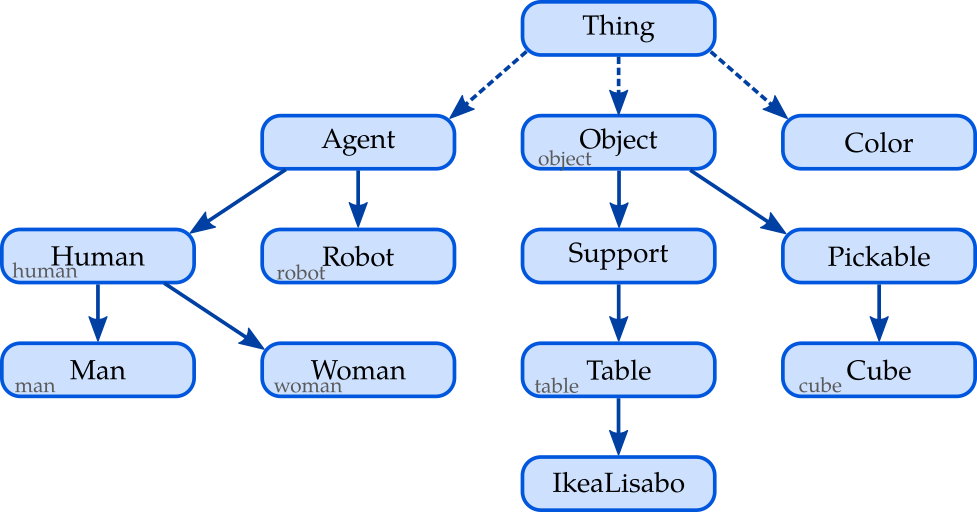
\includegraphics[scale=0.4]{figures/chapter2/Tbox.png}
\caption{\label{fig:Tbox} Representation of an ontology class hierarchy graph to illustrate the composition of a TBox. Taking the class Human, the bottom arrow has to be read as \textit{``A man is a kind of Human''}. The texts at the bottom left of the class are the classes' labels in natural language, when exist.}
\end{figure}

\improvement{Itemize}
The TBox $\Tbox$ contains assertions about the \textbf{classes} (types) of the ontology. It is defined by $\Tbox = \langle \classset, H \rangle$. It can be seen as a directed acyclic graph as presented in Figure~\ref{fig:Tbox}. $\classset$ is the set of all the classes of the ontology. In our example, $\classset = \{Thing,\ Agent,\ Object, ...,\ IkeaLisabo\}$. Considering the TBox as a graph, $H$ stores its directed edges. They represent the inheritance links between the classes (i.e. the subsumption assertions). We often use the special property ``isA'' to refer to these links (e.g. \textit{(Human, isA, Agent)}). In the OWL language, they are described with the property rdfs:subClassOf, as illustrated in the Listing~\ref{lst:Tbox}.

\noindent
\begin{minipage}{\textwidth}
\begin{lstlisting}[frame=single, basicstyle=\scriptsize\ttfamily, label={lst:Tbox}, caption={Description of ontology classes in the OWL language using the Turle syntax.},captionpos=b, style=OwlTurtle]
:Human rdf:type owl:Class ;
       rdfs:subClassOf :Agent .

:Man   rdf:type owl:Class ;
       rdfs:subClassOf :Human .
\end{lstlisting}
\end{minipage}

\subsubsection{The ontology RBox: Relations between Roles}

\begin{figure}[ht!]
\centering
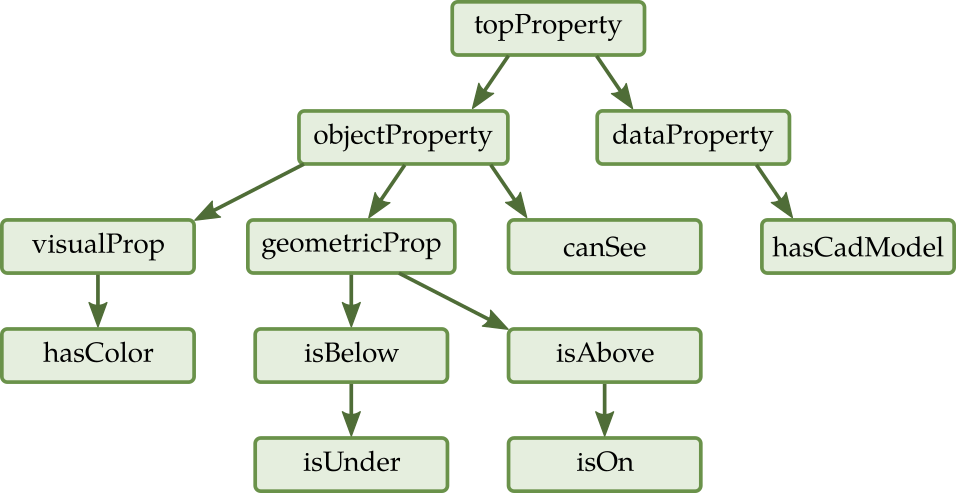
\includegraphics[scale=0.4]{figures/chapter2/Rbox.png}
\caption{\label{fig:Rbox} Representation of an ontology property hierarchy graph to illustrate the composition of an RBox. Taking the property isBelow, the bottom arrow has to be read as: \textit{``The property isUnder is a specification of the property isBelow''}.}
\end{figure}

The RBox $\Rbox$ contains axioms about the \textbf{properties} (roles). It is at least defined by $\Rbox = \langle \propset, \inclset, \invset, \domainset, \rangeset \rangle$. In the same way as the TBox, $\propset$ is the set of properties, and $\inclset$ stores the directed edges of the finite directed acyclic graph representing the inheritance links between the properties. Such a graph is represented in Figure~\ref{fig:Rbox}. These inheritance links aim at specifying properties. In our example, the property IsOn is a specification of the property isAbove in the way that an object being on another is an object that is above the latter and being in contact with. It is described with the property rdfs:subPropertyOf in the OWL language. 
$\invset = \{(\property, \property^{-1}) \in \propset^2\}$ is the set representing the properties inverses (\textit{e.g.} $(isOn, isUnder) \in Inv$). Describing the inverse of a property is useful first to reduce description work since if some describe a relation involving a property for which an inverse is defined, the inverse relation is also described in an underlying way. Moreover, for an algorithm exploring an ontology, knowing that a relation uses a property having an inverse can allow to reduce the algorithm complexity by not considering the inverse relation into the exploration.
Finally, $\domainset$ and $\rangeset$ are two sets representing respectively the properties domains and ranges. Their are define by $\domainset = \{(\property, \class)\}$ and $\rangeset = \{(\property, \class)\}$ with $\property \in \propset$ a property and $\class \in \classset$ a class. The domain of a property informs on the type of resources that may use the property, thus the type of the subject of a triplet. The range of a property informs on the valid values applied to the property, thus the type of the object of a triplet. For the property isOn, we would therefore have $(isOn,\ Object) \in \domainset$ and $(isOn,\ Support) \in \rangeset$. In this way, we state that the property IsOn can be used to describe that an object is on top of an object being support. Domains and ranges can be used in two ways. It can be to check the consistency of an ontology by checking if the way the properties have been used corresponds to their definition. It can also be used to reason on the ontology and extract new knowledge from a given situation. If, for example, an entity is said to be on top of another that is not described as being a support, we could deduce that this second entity may be a support.

The formalization above considers only a general kind of property while the OWL language makes the distinction between two main categories. The \textbf{object properties}, linking two entities, and \textbf{data properties}, linking an entity to a value. While both are slightly different, we will only keep a general definition of a property for our formalization to simplify the future algorithm explanations. An example of the description of an object property and a data property from the Figure~\ref{fig:Rbox} are illustrated in the Listing~\ref{lst:Rbox} using the OWL language.

\begin{lstlisting}[frame=single, basicstyle=\scriptsize\ttfamily, label={lst:Rbox}, caption={Description of ontology properties in the OWL language using the Turle syntax.},captionpos=b, style=OwlTurtle]
:isOn  rdf:type owl:ObjectProperty ;
       rdfs:subPropertyOf :isAbove ;
       owl:inverseOf :isUnder ;
       rdfs:domain :Object ;
       rdfs:range :Support .

:hasCadModel rdf:type owl:DatatypeProperty ;
             rdfs:domain :Object .
\end{lstlisting}

\subsubsection{The ontology ABox: Asserting facts}

\begin{figure}[ht!]
\centering
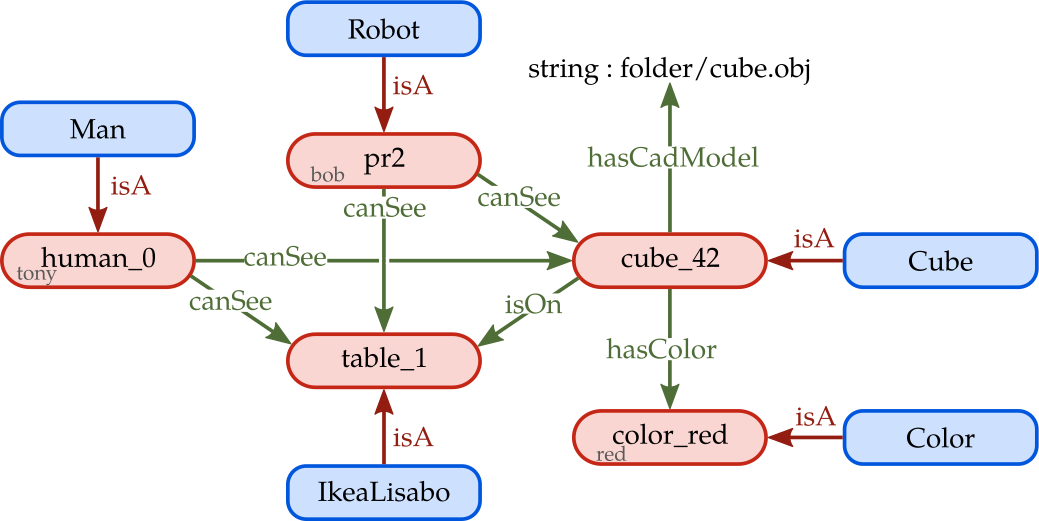
\includegraphics[scale=0.4]{figures/chapter2/Abox.png}
\caption{\label{fig:Abox}  Representation of an ontology instances graph to illustrate the composition of an ABox. Red boxes are individuals of the ontology. Green arrows are properties coming from the RBox and applied to individuals. Red arrows represent a direct inheritance link between an individual and a class coming from the TBox. The texts at the bottom left of the individuals are the individuals' labels in natural language, when exist.}
\end{figure}

The ABox $\Abox$ contains assertions about the \textbf{entities} (individuals) of the ontology. When we refer about entities, we no more speak about general concepts but rather of instantiated concept, being either a physic or virtual entity. The ABox is defined by $\Abox = \langle \indivset, \inheritset_0, \relationset \rangle$. $\indivset$ is the set of all the entities represented in the ontology. $\inheritset_0$ the set of direct types of $\indivset$ such as $\inheritset_0 = \{(\indiv, \class) \}$ with $\indiv \in \indivset$ an individual and $\class \in \classset$ a class. In the graphical representation of an ABox in the Figure.~\ref{fig:Abox}, the red blocks are the ABox entities ($\indivset = \{human_0,\ pr2,\ ...,\ table\_1\}$) and the red arrows with the label ``isA'' are the entities direct types ($(cube\_42, Cube) \in \inheritset_0$).
$\relationset$ is finally the set of \textbf{relations} between entities. Such relation are in the form of triplets $(\subject, \property ,\object)$ where $\subject$ is the subject, $\property$ the property and $\object$ the object. The set of relations is thus defined by $\relationset = \{(\subject, \property ,\object) | (\subject, \object) \in \indivset^2, \property \in \propset\}$. These relations are represented by the green arrows between the entities in Figure~\ref{fig:Abox}. We can note in this figure the presence of the use of a data property ``hasCadModel''. This property does not link two entities, which goes against the previous definition. Regarding our formalization and to keep it tractable, we can however keep it as it is, and view the string value as an entity having for direct type a concept ``String''. An example of the description of an entity from the Figure~\ref{fig:Abox} is illustrated in the Listing~\ref{lst:Abox} using the OWL language.

\begin{lstlisting}[frame=single, basicstyle=\scriptsize\ttfamily, label={lst:Abox}, caption={Description of an ontology individual in the OWL language using the Turle syntax.},captionpos=b, style=OwlTurtle_indiv]
:cube_42  rdf:type     :Cube ;
          :hasColor    :color_red ;
          :hasCadModel ``folder/cube.obj''^^string ;
          :isOn        :table_1 .
\end{lstlisting}

We just saw that in the ABox, $\inheritset_0$ contains the direct types of entities. We also saw that the classes can inherit from one another in the TBox, thanks to the classes inheritance directed edges stored in $H$. This means that the individuals of the ABox have inherited types. Taking the entity cube\_42 of Figure.~\ref{fig:Abox}, its direct type is the class Cube ($(cube\_42,\ Cube) \in \inheritset_0$). Regarding the TBox represented in Figure.~\ref{fig:Tbox}, a Cube is a kind of Pickable ($(Cube,\ Pickable) \in H$), itself being a kind of Object ($(Pickable,\ Object) \in H$). We can thus say that the entity cube\_42 is a Cube, a Pickable, and an Object. To represent it, we use $\inheritset$ to denote the set of direct and inherited types. We thus have $\{ (cube\_42,\ Cube), (cube\_42,\ Pickable), (cube\_42,\ Object)\} \subset \inheritset$.

\subsubsection{Extending the ontology TBox}

With the use of the relation set $\relationset$ of the ABox, we saw that we can apply properties to individuals to link them together and form relations in the form of triplets. However, some could want to apply properties to classes to describe general links between classes. While properties domains and ranges already give such relations this can be not enough. Taking an object property hasMother, we can assign to it the class Human for domain and Woman for range. With such description, we state that a human CAN have a mother, that is a woman. However, we do not describe that even if we do not know who it is, a human has a mother who is a woman. For this particular example, we could use cardinality constraint but we will not go as far. Taking now the data property hasCadModel of Figure~\ref{fig:Rbox}, we have applied it to a specific entity in the example of Figure~\ref{fig:Abox}. But what about a Table Lisabo (IkeaLisabo in Figure~\ref{fig:Tbox})? Any table of this model will have the same CAD model and we do not want to put this relation to every entity of this type. Here domains and range are not sufficient to represent it. To do so, we will use \textbf{annotation properties} applied to classes. Annotation properties are usually used to document ontologies and not to describe general relations on classes. We take thus some liberty regarding the OWL standard for convenience. However, we will try to use it in very particular cases where no other simple solution can be applied. Relations to classes using annotation properties are thus added to the definition of a TBox $\Tbox = \langle \classset, H, \annotationset \rangle$, where $\annotationset$ is the set of relation between classes in the form of triplets.

\subsubsection{Advanced use of properties}

In this sub-section, we present a formalism of an ontology in the form of $\kbs = \langle \Abox, \Tbox, \Rbox \rangle$. All the knowledge stored in $\kbs$ are sufficient to build exploration algorithm on top of it. However, to reason on ontology, additional descriptions are necessary in the form of properties characteristics. We do not add them to the knowledge base formalism but enumerate them below: 

\begin{itemize}
	\item \textbf{Symmetric property}: If the relation $(x, p, y)$ holds in $\relationset$ with $p$ being a symmetric property, the relation $(y, p, p)$ is also part of $\relationset$. \\ e.g. $hasSpouse$
	
	\item \textbf{Asymmetric property}: If the relation $(x, p, y)$ holds in $\relationset$ with $p$ being an asymmetric property, the relation $(y, p, p)$ cannot be part of $\relationset$. \\ e.g. $hasChild$
	
	\item \textbf{Reflexive property}: A reflexive property can be used to link an individual to itself. \\ e.g. $hasRelative$
	
	\item \textbf{Irreflexive property}: An irreflexive property cannot be used to link an individual to itself. \\ e.g. $hasParent$
	
	\item \textbf{Functional property}: Every individual can be linked by a functional property to at most one other individual. By this way, if ${(x, p, y), (x, p, z)} \subset \relationset$, then $y = z$. \\ e.g. $hasFather$
	
	\item \textbf{Inverse functional property}: Every individual can hold at most one inverse functional property. By this way, if ${(x, p, y), (z, p, y)} \subset \relationset$, then $x = z$. \\ e.g. $hasHusband$
	
	\item \textbf{Transitive property}: A transitive property describes a link between two individuals x and z whenever it exists a link between x and y, and y with z with this property. If ${(x, p, y), (y, p, z)} \subset \relationset$ with p a transitive property, then $(x, p, z) \in \relationset$. \\ e.g. $hasAncestor$
	
	\item \textbf{Property chain axiom}: While the transitive property characteristic decsribes a link between several individuals with the same property, the chain axiom does the same with distinct properties. Given the chain $p_1 \bullet p_2 \Rightarrow p_3$, if ${(x, p_1, y), (y, p_2, z)} \subset \relationset$, then $(x, p_3, z) \in \relationset$. \\ e.g. $hasParent \bullet hasParent \Rightarrow hasGrandparent$
	
	\item \textbf{Disjunction}: Given two disjoint elements (classes or properties), a third element cannot inherit of two disjoint elements. \\ e.g. $Man \sqcup Woman$
\end{itemize}

\subsubsection{Labeling functions}

We saw, in the previous chapter, that the semantic knowledge base is part of what we assimilate to be the declarative memory. The particularity of such memory is the ability to speak about the knowledge it stores. In this way, we introduce a labeling function $\labelfunc$ for any element of the ontology. This labeling function is specified for the individuals ($\alabel$), the classes ($\tlabel$), and the properties ($\plabel$). Considering the individuals labeling function $\alabel: \indivset \rightarrow Lbl$ with $Lbl$ a set of communicable names encoded as UTF8 string in our implementation. The same holds for the other two labeling functions.

\subsubsection{Ontology for Human-Robot Interaction}

Because we are working in the field of Human-Robot Interaction, it is mandatory for the robotic agent to be able to represent its own knowledge but also to represent an estimation of its human partners' knowledge. Such features will be explained later in this thesis and we only introduce the related notation for the moment.
We define the robot's own symbolic knowledge base $\kbs^R = \langle \Abox^R, \Tbox^R, \Rbox^R\rangle$.
Then, for each human agent $H_i$ the robot knows, we consider the agent's semantic knowledge $\kbs^{H_i} = \langle \Abox^{H_i}, \Tbox^{H_i}, \Rbox^{H_i} \rangle$.
The robot's global knowledge thus encompasses both its own semantic representation of the environment as well as an \textbf{estimation} of the other agent's knowledge.
In the rest of this thesis, we will simply use the notation $\kbs$ in cases where the used knowledge base does not matter (i.e. either the robot one or an estimated one can be used).

\subsubsection{Ontology formalism recap}

The ontology definition used all along this thesis is summarized in Table~\ref{tab:onto_symboles}.

\begin{table}[ht!]
\caption{The list of symbols used to define a semantic knowledge base as an ontology }
\label{tab:onto_symboles}
\begin{tabular}{ll}
{\ul \textbf{$\Abox$ ABox entities/indiv}} & {\ul \textbf{$\Tbox$ TBox classes/concepts}}  \\
$\indivset$: set of entities               & $\classset$: set of classes  \\
$\inheritset_0$: entities' direct types        & $H$: classes inheritance links \\
$\relationset$: relations between entities    & $\annotationset$: relations between classes  \\
$\alabel$: individuals labeling function & $\tlabel$: classes labeling function \\
 & \\
\multicolumn{2}{l}{{\ul \textbf{$\Rbox$ RBox roles/properties}}}                          \\
$\propset$: set of properties              &                                              \\
$\inclset$: properties inheritance links       & $\invset$: properties inverses                   \\
$\domainset$: properties' domains sets     & $\rangeset$: properties' ranges sets   \\
$\plabel$: properties labeling function & \\
\end{tabular}
\end{table}

\section{Architecture}

Now we have presented what an ontology is and the desired features for a software managing a \acrfull{kb} based on an ontology, we introduce the resulting software, Ontologenius. In this section, we start with the software architecture able to manage a single ontology instance, meaning the \acrshort{kb} of a single agent. The goal of this section is not to go deep in the technical implementation but rather to give cues to understand how the \acrshort{kb} is managed.

The architecture of Ontologenius is divided into three major modules as shown in figure~\ref{fig:chap2_archi_single}: the knowledge storage (permanent and temporary data structures), the \acrshort{kb} exploration (transient data) and the reasoning (plugins). Ontologenius has been developed in C++14 and is based on ROS for the communication layer and the plugins management. It is compatible with ROS Kinetic (2016), Melodic (2018), and Noetic (2020). 

\begin{figure}[ht!]
\centering
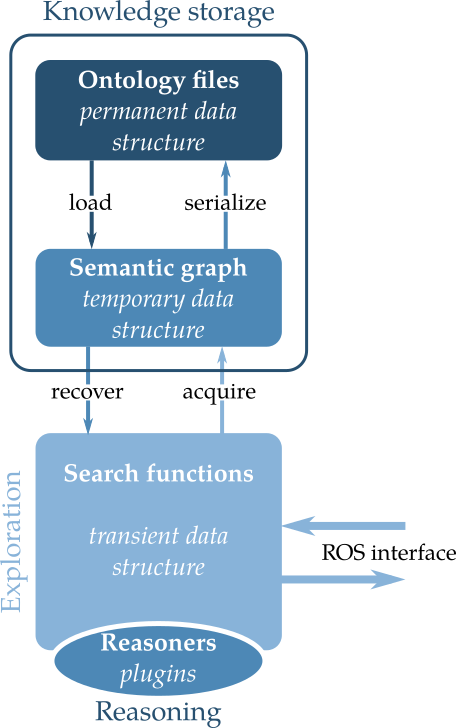
\includegraphics[scale=0.5]{figures/chapter2/archi_single.png}
\caption{\label{fig:chap2_archi_single} The software architecture of Ontologenius to manage a single \acrlong{kb} in the form of an ontology.}
\end{figure}

In this section, we first explain how ontology files are loaded and converted into a semantic graph. Then, we present the available reasoners and their management. Finally, we explain how the system deals with natural language name.

\subsection{Permanent versus temporary data structure}

To store the \acrlong{kb} as an ontology, we first use OWL files using the XML/RDF syntax. The files can be read from a local folder on the computer or retrieve from the internet. Ontology files often include others, as an upper ontology. However, Ontologenius is not able for now to solve these dependencies. All the required files thus have to be listed. These files are what we consider to be a permanent data structure. Nevertheless, our goal is not just to load a static \acrlong{kb}. This latter aims to be updated all along an interaction and if the robot learns new concepts, we want it to be able to memorize them for the next interaction. In the same way, if the robot interacts with a given agent and estimates him to know some concepts, it needs to memorize them for the next interaction with this specific agent. Consequently, we consider two kinds of files. On one hand, we have what we call the inputs files, being a default \acrlong{kb}. On the other hand, we have the internal file, being the \acrlong{kb} of a given agent. Their management is illustrated in figure~\ref{fig:chap2_files}. If no internal file exists for the managed agent, the input files are loaded (a). This will be the case for the first time we start the robot if the \acrlong{kb} is the robot's one, or the first time the robot interacts with a new agent if the \acrlong{kb} is an estimation of an agent \acrlong{kb}. The input files thus represent the minimal knowledge we estimate an agent to have. Once we power off the robot or when an agent leaves an interaction, all the maintained \acrlong{kb} is serialized into a single OWL file, the internal file. This file is thus a backup of an agent's \acrlong{kb}. The next time the robot is powered on, or the next time it interacts with a known agent, the internal file is load and the input files are no more considered (b). The robot can thus refine its estimation of the others knowledge as well as its own knowledge over interactions.

\begin{figure}[ht!]
\centering
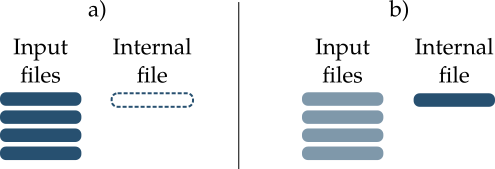
\includegraphics[scale=0.6]{figures/chapter2/files.png}
\caption{\label{fig:chap2_files} a) In case no intern file already exists, The input files are considered as the default \acrlong{kb} of the agent b) In case an internal file exists for a given agent, this means that the robot already interact with this agent. In this latter case, the input files are not considered and the agent previously estimated \acrlong{kb} is loaded. If the current \acrlong{kb} represents the robot's one, the robot just restarts with its previous \acrlong{kb}.}
\end{figure}

When ontology files are loaded, they are converted into a kind of semantic graph, at the difference of triple store. Each element of the ontology (individuals, classes, object properties, and data properties) are represented as nodes. We thus have four types of nodes. The nodes have several set of pointers toward other nodes, each having a semantic meaning. Such a representation is useful for efficient search algorithms like query resolution. For example, wanting to know all classes from which an individual inherits, from the node of this individual, we just have to iterate over all the nodes in the set of inheritance and perform recursion on each of them, iterating once again on the set of inheritance.

To find the entry point of the graph, we have four containers, one for each element type. These containers provide an efficient retrieve of an element from its identifier. In addition, the containers provide readers-writer lock mechanism, allowing concurrent access for ready-only operation while ensuring exclusive access for a write operation. Thanks to this synchronization primitive, Ontologenius is thread-safe.

\subsection{Reasoning to enrich the knowledge}

Reasoning on a \acrlong{kb} is a primal need to extract new knowledge from the described one. At the difference of tableau algorithm~\cite{zuo_2006_high}, we do not want to create a dedicated model to do so. Consequently, we made the choice to develop our own reasoners, able to run on the Ontologenius internal representation.

The reasoners are implemented on the basis of plugins for an easy extension. The proposed plugin interface allows the execution of reasoning processes either before the resolution of a query, after an update of the \acrshort{kb}, or periodically. The reasoners are not necessarily limited to first-order logic. Users can implement any process depending on their needs. To date, we have four usual reasoners to solve the symmetric properties, the inverse properties, to reason on domain and range, and to solve chained axioms. We have also implemented a reasoner dedicated to the proposition of complementary labels and another to create relations on classes, using annotation properties, being generalization of the existing relation. For example, if several entities own relation toward the same CAD model file, the reasoner will generate a relation toward this CAD model to an upper common class to all these entities.

A YAML configuration file can be provided to choose the reasoners to use and to tune each reasoner depending on the application. Any available reasoner could also be activated and deactivated at run time.

To avoid time loss during reasoning, two mechanisms are available. For the reasoners needing to run once on each element, they can mark the elements on which they have run. By checking these marks they can know if an element has already been analysed or not. The second can be compared to a to-do list. Any element owns an update flag. When an element is modified by an external process, like a perception process, the flag of the element is raised. Reasoners then run only on the elements having this flag raised. If they find a new relation to insert in the \acrshort{kb}, they can raise the flags of the impacted elements. The other reasoners will thus check again for these newly updated elements. A reasoning pass ends when no more update has been performed by any of the reasoners.

Finally, to facilitate the deletion of inferred relations, we attach a reference to any relations that have allowed those inferences. In this way, by removing a relation, we are able to find side relations that also need to be removed. For example, consider the chain axiom $isIn \bullet isOn \Rightarrow isOn$. If A isIn B and B isOn C, the reasoners will generate the relation A isOn C. The two former relations have thus allowed the inference of the latter. If one of them is removed, the third also has to be removed. If A is no more in B, it is consequently no more on C. In this way, the \acrshort{kb} can always be kept up to date without performing reasoning from scratch at each update, neither by creating a side model dedicated to the reasoning. However, it is less efficient than classic reasoning methods which can use dedicated models.

\subsection{Concepts' name in natural language}

Having labels attached to elements is quite usual. As others, Ontologenius attaches to any element a map linking a country-language code to a set of labels. The slight difference of Ontologenius is that it supports a special kind of labels, called muted labels. They are labels that are only used to retrieve an element from it but that can not be retrieved from an element. For \acrshort{hri} application, it allows the robot to understand some words but to not use them when it speaks. For example, for the restaurant Mac Donalds, we want the robot to understand ``Mickey D's'' in the US, ``Mekkes'' in Germany, or ``McDo'' in France. However, we prefer the robot to use the true name.

\section{Managing others' estimated knowledge}

A major feature of Ontologenius is the ability to manage several ontology instances, to represent both the robot's knowledge and the estimation of its partners' knowledge. In this section, we first present how the multiple instances are managed by Ontologenius. We then present two advanced uses: the deep copy of an instance and the representation of multiple knowledge state in a single instance.

\subsection{Ontologenius multi-instances principle}

What we refer to when we use the term instance is an instantiation of the previously presented architecture. It thus represents a single \acrlong{kb} being either the one of the robot or an estimation of the \acrlong{kb} of one of its partners. To manage multiple instances, we use the architecture represented in figure~\ref{fig:chap2_archi_multi}.

\begin{figure}[ht!]
\centering
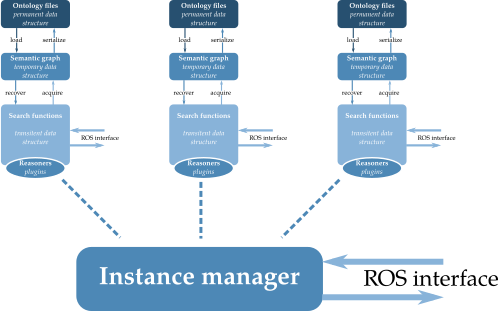
\includegraphics[width=\textwidth]{figures/chapter2/archi_multi.png}
\caption{\label{fig:chap2_archi_multi} The software architecture of Ontologenius to manage multiple \acrlong{kb}s in the form of an ontology. An instance manager makes the link between each instance and has a direct access to each semantic graph to propose queries. }
\end{figure}

The architecture of each instance stays the same as previously, this means that each instance has its own ROS instance and can be queried and updated independently. However, to not just manually run several instances and not have any conflict on the ROS topics and services names, we add an instance manager. This manager owns all the instances and can create new ones as well as deleting existing ones. In addition, it attributes an identifier to each instance. It is often the identifier of the agent it represents. With this identifier, each instance creates dedicated and non-overlapping ROS services and topics. The manager itself owns a ROS interface to perform the deletions and creations.

When a new instance is created, it runs in a dedicated thread. Consequently, having multiple instances does not slow down Ontologenius. The manager keeps a reference to the instance and can have access to the knowledge of each of them without passing by ROS. It allows the manager to propose queries involving several instances. For example, the only existing one for the moment computes the difference of knowledge between two instances, about a given entity. With such direct access to the semantic graphs, it allows easy and efficient belief divergence checking.

Finally, because each instance has an identifier, when one is killed, it stores the maintained knowledge in an OWL file referenced with this identifier. Consequently, when an instance is started, it can automatically load the previous state of the \acrshort{kb}, using the instance identifier.

\subsection{Catching knowledge at a given moment}

The instances representing the robot's \acrshort{kb} and the estimation of its partners' \acrshort{kb}s aim to be continuously updated by perception processes. However, some processes, like task planning, need a stable version of a \acrshort{kb}. In addition, some processes like (once again) task planning may need to modify a \acrshort{kb} to represent future possible states. Nevertheless, if a process modifies the same \acrshort{kb} that is updated by the perception, it would neither represent the future state, neither the current states.

To avoid such a situation, Ontologenius provides a mechanism to copy an instance. It performs a deep copy, keeping all the inferred knowledge, the inference traces, or the reasoners' configurations. The resulting instance becomes completely independent from the previous one and can be modified without altering it.

The only difference is that an instance resulting from a copy will not be saved into an OWL file when it will be deleted. It is a draft, to test possible state.

\subsection{Exploring several possible mental states at once}

Having a dedicated instance to represent possible futures is useful, however planning processes could need to maintain multiple states at a time. A deep copy is far from being a free operation as presented in the result section of this chapter. It takes time, especially for large \acrshort{kb}s. Moreover, we cannot imagine to maintain too many instances at the time\footnote{From our unlucky tests, the process died after the creation of 82 instances with small knowledge bases.}.

To face this issue, we propose with Ontoogenius a kind of versioning system. First of all, this system is only available on instances resulting from a copy, as the others do not aim to represent multiple states. Taking the term of the git versioning system, we perform some modifications on a \acrshort{kb} and all the changes are tracked. When we consider that all the changes represent a version, we perform a commit. This commit has an identifier, and a parent commits. Wanting to go back to a previous version of the \acrshort{kb}, we can checkout this version thanks to the identifier. The versioning system thus applies the modifications in the inverse order to create the previous state. From there we can thus have multiple version of the same \acrshort{kb} but it only represents a linear evolution. Most of the planning systems work with branching, allowing from one state to imagine multiple future states. Where git would use branches also, with ontologenius, we do not and we can simply perform a new commit on an old one. It automatically creates a new branch without explicit management of it. We can thus easily checkout a commit of another branch. However, once a branch is created, it will never be possible to merge it with another one. Consequently, it creates a tree.

From the commit identifier, the users are free to set it or to let Ontologenius setting it.

\begin{figure}[ht!]
\centering
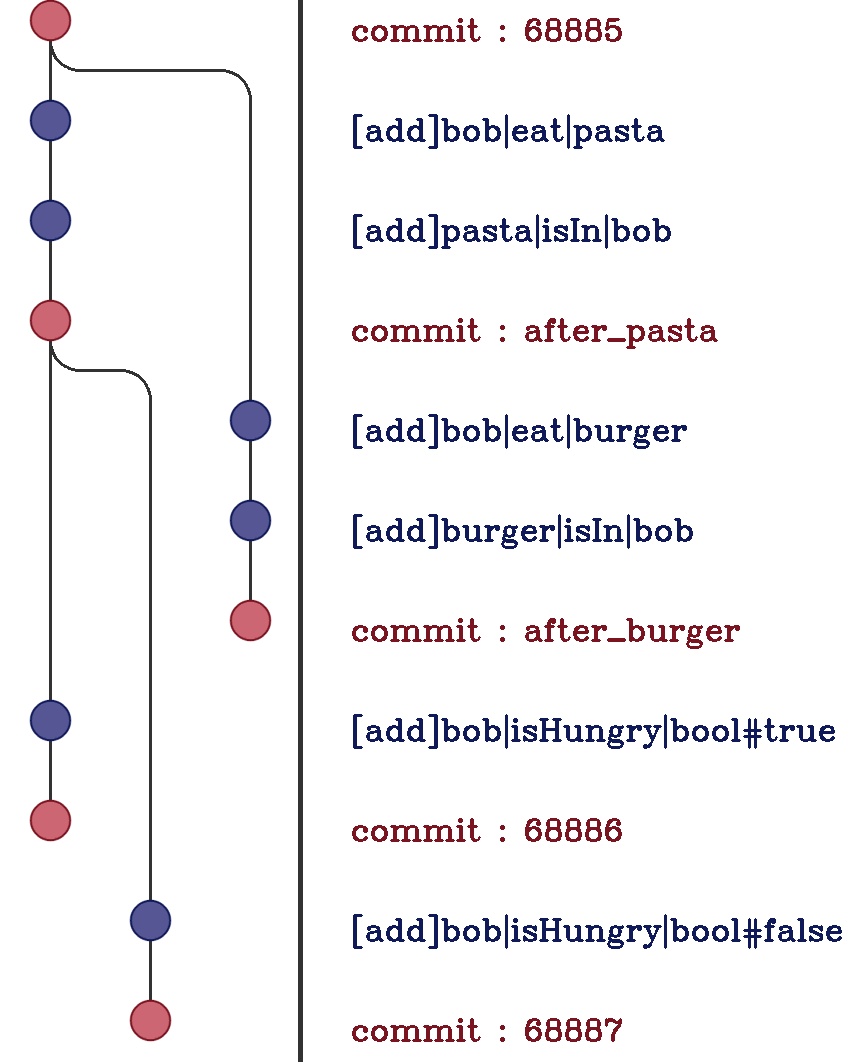
\includegraphics[scale=0.22]{figures/chapter2/commit.png}
\caption{\label{fig:chap2_commit} An example of a versioning tree drawn with Ontologenius. In red are the commits and in blue the changes. The temporal order of the operations is respected from top to bottom. }
\end{figure}

Finally, for debug purpose, Ontologenius can generate an XML file representing all the versioning, with the commits and the changes. An executable allows then to generate an image of it to understand what an algorithm has performed. An example of such an image is presented in figure~\ref{fig:chap2_commit}.

\section{Using Ontologenius in robotic applications}

Now we explain Ontologenius architecture and its management of the instance, in the current section, we present how to use it once it is launched. We explain how knowledge is inserted at run-time and how knowledge can be retrieved. Finally, we present tools to facilitate its use with API and GUI.

\subsection{Updating the knowledge base}

To represent the state of an evolving environment, updating the \acrshort{kb} is a key feature for software managing \acrshort{kb}. First of all, the update process is asynchronous in Ontologenius. Updates are filled in an internal buffer which is periodically analysed. For a usual instance, updates are looked up at 20hz. Such a frequency is sufficient for updates coming from perception processes. For instances coming from a copy, the update process runs at a higher frequency of 1000hz, meaning that a published update will start to be processed at most 1ms after its publication. The need for a higher frequency for instances coming from copy is due to their aim. The goal of such instances is to make a caption of the state of a \acrshort{kb} at a given instant and then to freely modify it to run an external process like task planning. A delay of 50ms would not be acceptable for this kind of process. Once the update process is triggered by a non-empty buffer, it runs until the buffer is empty. In this way, even if a lot of updates are published at once, no additional delay is introduced.

Since the updates are asynchronous but that some components may need to be sure that all updates have been applied before continuing, Ontologenius raises a signal once it has no more update to process. Before rasing this signal Ontologenius also applied all the needing reasoning so that the \acrshort{kb} is consistent and populates with all the inferred knowledge. It allows a synchronisation for components needing it, to start a new process on a stable \acrshort{kb}.

The content of a single update is composed of an operator, either an addition or removal, and a triplet. In the current version, the triplet can be relations to individuals using object or data properties, relations to classes using annotation properties, inheritance links, inverse axioms on object properties, or labels to any elements. At least the subject or the object of the triplet must be already known by the system to apply the update. ALL the other elements are created with a deduction of their types (i.e. individual, class, property).

If the content of an update is a removal, all the inferences made on the basis of the original triplet are removed too. In addition, for any update, the related triplet is republished on another topic with a timestamp. For the inferred triplet, they are published by Ontologenius on a dedicated topic with a reference to the triplets having been used to perform the inference or to remove it. It allows, if needed, temporal storage of all the updates of the world with a temporal consistency about the inferred knowledge. This means that even if the knowledge has been inferred later than the original knowledge update, it is possible to temporally align them.

\subsection{Retrieving knowledge}

To retrieve knowledge from Ontologenius, two ways are available. The main query system consists in a set of low-level and parametric queries for precise and efficient retrieval. The second system is based on a more classic RDF query language that is \sparql{}.

\subsubsection{Low-level queries}

The principal query system proposed by Ontologenius is a set of low-level queries organized around the four main types used in the ontology: the individuals/entities, the classes/concepts, the object properties, and the data properties. For each of these types, dedicated queries are available.

First, all four types have 10 common queries related to the exploration of the upper hierarchy and the names in natural language. We will not review them one by one but rather take two of them to give an indication of their composition and functioning. 

\begin{verbatimtab}
string getName(string uri, 
               bool take_id = true);
\end{verbatimtab}

The getName query allows a user to retrieve one of the labels of a given element. If the element has multiple labels, one is selected randomly. This query is impacted by the general language configuration. If Ontologenius is configured to work in English, only English labels will be retrieved. The language configuration can be changed at run-time. This query has an optional parameter take\_id. If it is set to true, if the queried element does not have labels, its id can be used as a default label, regardless of the language setting. 

\begin{verbatimtab}
vector<string> getUp(string uri,
                     int depth = -1, 
                     string selector = ``'');
\end{verbatimtab}

The getUp query allows a user to explore the upper hierarchy of a given element. By setting only the mandatory parameter, it returns all the elements for which the given element inherits. If A inherits from B and B from C, interrogating the hierarchy of A will give B and C. With the depth parameter, the user can set the depth exploration. Setting it to 1, the query will only return the direct hierarchy. The last optional parameter, the selector, can be used to filter the results to be returned. Among the returned elements, Ontologenius will only keep the ones inheriting from the selector. Wanting to know if entity A is of type B, one can query a getUp on A with B as the selector. If the result is empty, A does not inherit B.

To query individuals, Ontologenius provides 14 additional queries. We can query for the properties applied to a given entity, the entities it is linked with, the properties it is range of, etc. Most of them support the optional parameters of depth and selector.

For the classes, we have 13 additional queries. We can explore the relations using annotation properties, get the classes inheriting from a given one, get the properties for which it is domain of, etc.

For the object properties, we have 5 additional queries. We can know their domain and range, their inverse, their disjunction, or their hierarchy. For the data properties, we have the same excepted the inverse.

\subsubsection{SPARQL-like queries}

The low-level queries provide a fine and efficient exploration of the \acrshort{kb}. Encouraging the user to select the right query depending on its need, Ontologenius does not have to perform analysis on the query itself to find how to resolve it. However, such queries can be difficult to use in a first time and is not adapted to every usage. Consequently, with Ontologenius we also provide a \sparql{}-like query interface.

\sparql{}, for \sparql{} Protocol and RDF Query Language, is a semantic query language for databases. A \sparql{} query looks like:

\begin{minipage}{\textwidth}
\begin{verbatimtab}
SELECT ?name 
       ?email
WHERE
  {
    ?person  a     Person .
    ?person  name  ?name .
    ?person  mbox  ?email
  }
\end{verbatimtab}
\end{minipage}

Through the SELECT keyword, we first specify the variables we want to get the possible binding. Here we ask for pairs of names and emails. With the WHERE block, we explain the conditions to respect in order to fill the variable. It is the query pattern. In the provided example, we define a variable (always prefixed with a question mark) person which should be of type Person. Then, for all the possible value of the variable person, we retrieve their name and email. With the SELECT keyword, we can specify a sub-set of the involved variable to be returned.

Three other keywords can be used instead of SELECT. It exists CONSTRUCT, ASK, and DESCRIBE. In addition, we can apply filters or aggregation rules. \sparql{} is a really rich language but we have chosen to take the minimum as it is not the main entry point of Ontologenius.

Consequently, Ontologenius only implements the SELECT query variation with the pattern in the WHERE, as a list of triplets. Nevertheless, we have added the keyword DISTINCT, optional after the SELECT, which ensure to only retrieve distinct results.

In the rest of this thesis, and for better readability, we only write the patterns of the \sparql{} queries when we present some.

\subsection{Interfacing with Ontologenius}

To work with Ontologenius in the easiest way as possible, we provide to the users several tools. Here we present the Application Programming Interface (API) and the debugging Graphical User Interface (GUI).

\subsubsection{The Application Programming Interfaces}

To provide an abstraction of the ROS middleware, and thus of the ROS messages, we propose two API to use Ontologenius. One is in C++\footnote{\url{https://sarthou.github.io/ontologenius/cpp_API/CppAPI.html}} and the other in Python\footnote{\url{https://sarthou.github.io/ontologenius/python_API/PythonAPI.html}}. Both are constructed in the same way and use approximately the same methods names to easily go from one to the other depending on the needs. They are composed of 13 classes for a total of more than 90 distinct methods. Such a number of methods allows a fine and precise use for the instance management, the reasoners' management, the knowledge insertion, or the ontology query. In addition, the methods support all the exploration options in an intuitive way.

The API also takes advantage of advanced ROS use for the services. It provides a direct TCP connection with a recovery mechanism. For intensive query use in a limited time, the first query will take more time to establish a direct connexion and all the following will benefit from it. It thus provides efficient and safe communication without additional complexity for the users.

Finally, to take Ontologenius and its APIs in hand, Ontologenius comes with five tutorials\footnote{\url{https://sarthou.github.io/ontologenius/cpp_Tutorials/Tutorials.html} and \url{https://sarthou.github.io/ontologenius/python_Tutorials/Tutorials.html}} covering its more basic usage to the more complex ones including the use of the versioning mechanism.

All the APIs description and the tutorials are available online on a website dedicated to Ontologenius: \url{https://sarthou.github.io/ontologenius}.

\subsubsection{Debbuging tool}

\begin{figure}[ht!]
\centering
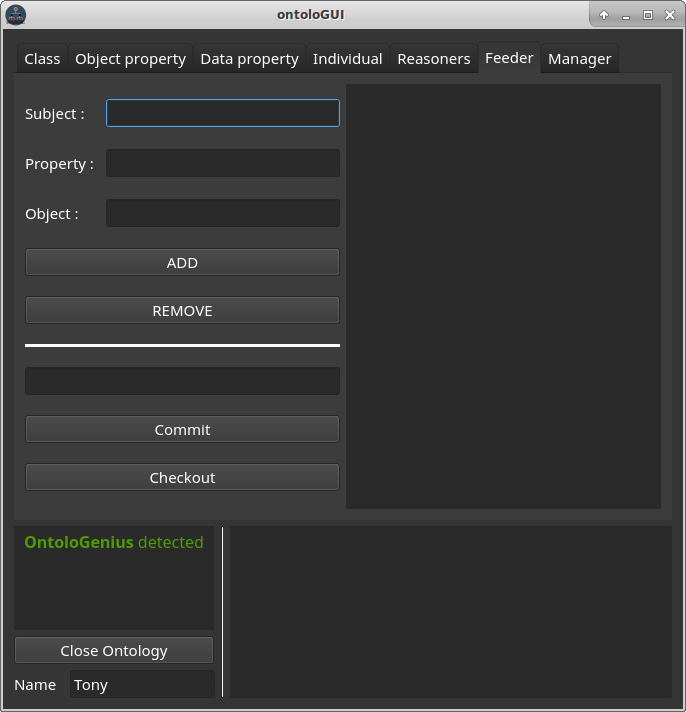
\includegraphics[scale=0.48]{figures/chapter2/ontologui.png}
\caption{\label{fig:chap2_ontologui} A view of the Ontologenius Graphical User Interface. With the displayed panel a user can insert or remove triplets from a given instance. On the left-hand bottom, we can see that the current instance is called Tony.}
\end{figure}

To help new users to take in hand Ontologenius and to help more experienced users to debug their applications using Ontologenius, we provide a Graphical User Interface (GUI). It has been developed using Qt. It is linked to ROS and provides almost all the methods available with the API like the instance management, the reasoners' management, the knowledge insertion, and the ontology query. In addition, for all the exploration queries, hovering a button provides a brief explanation of the hovered method and its equivalent in the ROS command lines.

In this chapter, we saw that Ontologenius is based on a lot of low-level queries for a precise and efficient exploration of an ontology. This GUI is thus often used during the development of an application using Ontologenius to choose the right method to use by allowing the developer to directly test the kind of results he can expect with a given query. In addition, at run-time, developers can easily explore the \acrshort{kb} to understand the origin of bugs in their application.

\section{Computational preformance evaluation}

In this section, we evaluate the Ontologenius performance and scalability through comparison with two systems and using their own tests. First, we compare with the KnowRob system with a focus on required CPU time to insert new knowledge and required memory to store this knowledge. The second system is ORO. With this latter, we measure query resolution time. Finally, we present some additional measurements like concept recovery time and deep-copy time.

\subsection{Comparing with Knowrob}

We start these comparisons with the KnowRob system presented in~\cite{tenorth_2013_knowrob}. This system is composed of several modules able to perform dedicated reasoning like temporal reasoning, CAD model segmentation, or object perception. All these modules are integrated around the logical programming language SWI Prolog~\cite{wielemaker_2012_swi}. OWL ontologies are loaded using the SWI Prolog’s Semantic Web library~\cite{wielemaker_2003_prolog} which provides an efficient and scalable way to manipulate RDF structures in Prolog. Internally, the triplet structure of the ontologies is represented as Prolog predicates. At the difference of Ontologenius, the Prolog system and thus KnowRob does not aim to be used as a server but rather as a monolithic and highly integrated system. To provide a fair comparison, in the part, we use Ontologenius without the ROS communication layer. Consequently, a single process runs both Ontologenius and the test application.

\cite{tenorth_2017_representations} proposes a detailed presentation of the internal representation of KnowRob and presents some performance and scalability analysis. The following comparisons have to be considered carefully. KnowRob is a wider and more mature system than Ontologenius. It proposes more advanced capability in terms of reasoning and integration. Ontologenius is more focused on \acrshort{hri} applications as presented earlier in this section. In this way, some simplifications that have been done to fit at our best the KnowRob tests may impact the results. The final reason why the following results should be taken with caution is that due to the complexity of the KnowRob system, we did not perform their test on our end. The results for the KnowRob system comes from their paper~\cite{tenorth_2017_representations}. Consequently, in this section, we do not aim to show that Ontologenius is ``better'' than KnowRob. We rather want to show that Ontologenius is not out of scope in terms of performance and scalability regarding a well-established software.

For the tests we have replicated, they use the description of visual perception entities. Such an entity represents the occurrence of the perception of a given object, having a given pose at a given instant. An example of one of these entities is illustrated in listing~\ref{lst:chap2_visual_perception}. The entity $cup\_i$ is the perceived object. The entity $VisualPerception\_i$ is the perception occurrence. It uses an object property to make a link with the perceived object and two data properties to represent the object's pose and the perception time stamp. The first simplification we had to make is the representation of the matrix of position. In Ontologenius, the data types are only represented in a serialized way as no internal manipulation of these types are made. Thanks to the use of Prolog, KnowRob can manipulate such a matrix and perform operations on it. Even if it is not said if they have inverse properties or not, we add one for the \textit{objectActedOn} property in order to know in which perception instance an object has been perceived.

\begin{lstlisting}[frame=single, basicstyle=\scriptsize\ttfamily, label={lst:chap2_visual_perception}, caption={Description of a visual perception entity created in a comparable way as in the KnowRob system. The description is provided in the OWL language using the Turtle syntax.},captionpos=b, style=OwlTurtle_indiv]
:cup_i  rdf:type   :Cup ;

:VisualPerception_i  rdf:type         :VisualPerception ;
                     :objectActedOn   :cup_i ;
                     :eventOccursAt   [[1,0,0,2.56], ... ,[0,0,0,1]]^^RotMat ;
                     :startTime       6572^^Time .
\end{lstlisting}

\begin{figure}[ht!]
\centering
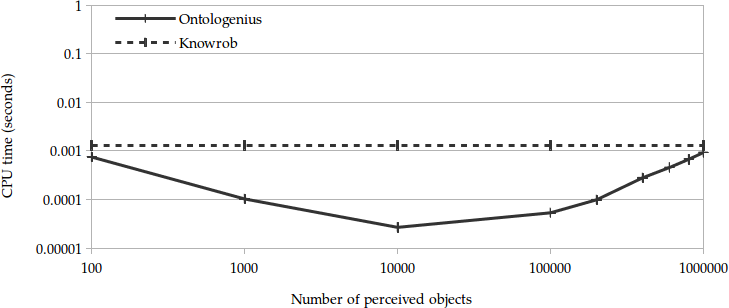
\includegraphics[width=\textwidth]{figures/chapter2/knowrob/Insertion.png}
\caption{\label{fig:chap2_knowrob_insertion} Comparison of the required CPU time for creating large numbers of object perceptions in the knowledge base. Each inserted object correspond to a visual perception entity linked to a cup, a pose matrix, and a time stamp. Ontologenius is used without the ROS communication layer to provide comparable usage and thus results.}
\end{figure}

The first test consists of creating and inserting N visual perception entities in the \acrshort{kb} and measuring the required CPU time to insert one of them. This means that we measure the average CPU time over N insertions. For each visual perception entity, we thus have to create two entities (the visual perception entity and the perceived object), two inheritance links, two raw data, and three relations (two based on data property and one based on object property). The results are shown in figure~\ref{fig:chap2_knowrob_insertion}. KnowRob has a constant insertion time around 1.3ms. With Ontologenius we do not have constant time. The first decreasing part can be explained by the asynchronous Ontologenius mechanism. It looks for updates at 20hz. Consequently, we can have a delay between the moment we publish updates and the moment they are processed. The effect of the mechanism disappears with the amount of data to process since once the update mechanism started, it does not stop while data have to be processed. The general trend is thus an increase in the required CPU time. This increase can come from the fact that Ontologenius performs reasoning, like the creation of the inverse relations, at update where KnowRob resolves it at query. In addition, Ontologenius also performs consistency check at update. However, until 1,000,000 insertions and thus 2,000,000 of entities, 2,000,000 raw data, and 5,000,000 triples (2 for inheritances and 3 for relation per perception entity), the required CPU time is under 1ms.

Considering the same insertions as previously, the second test consists of measuring the required memory. The results are shown in figure~\ref{fig:chap2_knowrob_memory}. For a high number of individual, Ontologenius required a bit less memory. It can be explained by the fact that it has a simplified matrix representation. In addition, no information had been provided about the initial content of the~\acrshort{kb}. Both systems, therefore, require memory in the same order of magnitude.

\begin{figure}[ht!]
\centering
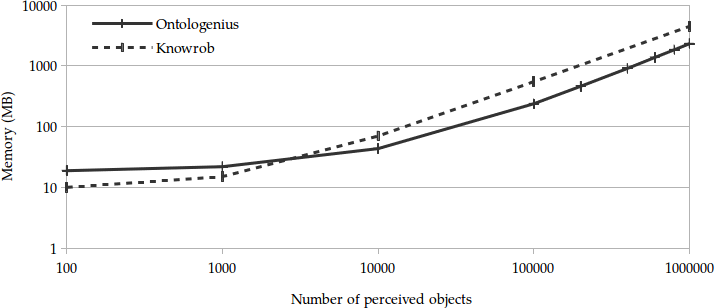
\includegraphics[width=\textwidth]{figures/chapter2/knowrob/Memory.png}
\caption{\label{fig:chap2_knowrob_memory} Comparison of the required memory for creating large numbers of object perceptions in the knowledge base. Each inserted object correspond to a visual perception entity linked to a cup, a pose matrix, and a timestamp. Ontologenius is used without the ROS communication layer to provide comparable usage and thus results.}
\end{figure}

The last test with KnowRob is about the required CPU time to perform queries. They took the same \acrshort{kb} as made previously, with N visual perception entities. The goal here is to select randomly one of the perceived cups, then retrieve its pose. In Prolog, the query is:

\paragraph{?-} owl\_individual\_of(Obj, kr:’Cup’), current\_object\_pose(Obj, Pose).

Using the low-level queries of Ontologenius, we have made a function doing the equivalent. It requests for all the cups, selects one randomly, retrieves the visual perception entity it is linked to, and fetches the pose. The required CPU time is reported in figure~\ref{fig:chap2_knowrob_query}.

\begin{figure}[ht!]
\centering
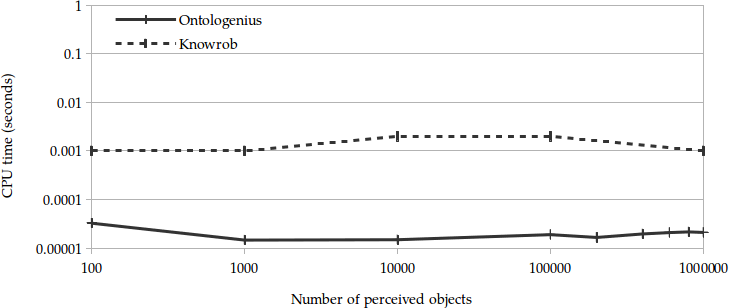
\includegraphics[width=\textwidth]{figures/chapter2/knowrob/Query.png}
\caption{\label{fig:chap2_knowrob_query} Comparison of the required CPU time for querying the pose matrix of a randomly selected object after that N perception entities have been created. Ontologenius is used without the ROS communication layer to provide comparable usage and thus results.}
\end{figure}

Concerning KnowRob, the query time is almost constant, jumping between one and two milliseconds. It has to be noted that in Prolog, the time measurement resolution is about 1 millisecond. Nevertheless, due to the jump, we can assume that the real value is not far from the millisecond. For Ontologenius, the query time is also almost constant, with values around 0.02ms. This significant difference, with an average factor of 75, can be due to the more precise queries provided by Ontologenius and to the fact that Ontologenius does not have to solve inference at query time. For the more precise queries, submitting a query to Prolog, KnowRob has to perform a kind of search among the \acrshort{kb} to make the submitted predicates true. At the difference, Ontologenius requires the programmer to refine and decompose the high-level query, allowing the execution to be more efficient. For the inference, most of the relations are inferred at the update, like the ones coming from inverse properties. At query, Ontologenius only has to go through the existing relations and only reasons about the classes and properties inclusion axioms. For example, if we had a query for all the objects, no direct link would have been created between the cups instances and the object class, this part would thus have been solved at query thanks to exploration.

In light of the presented results, even if both software have not the exact same goal, way of use, and maturity, we can at least conclude that Ontologenius is not out of scope with acceptable performance and scalability. Since Ontologenius provides fewer functionalities or at least different ones, the results are encouraging.% Having poor results with fewer functionalities would have been more problematic.

\subsection{Comparing with ORO}

For the second comparison, we select the software ORO~\cite{lemaignan_2010_oro}. At the difference of KnowRob which does not address the same \acrshort{hri} applications, ORO does. It works as a central server, usable by all the components of architecture and is able to manage several instances at a time. In this way, it has been designed for \acrshort{hri} applications. We can however note three major differences from a technical point of view. It is based on the Jena framework for the RDF triplets storage and uses Pellet~\cite{sirin_2007_pellet} for the reasoning part. Pellet supports OWL-DL expressiveness level to perform reasoning where with Ontologenius we are still at the OWL-lite expressiveness. Regarding the way to query the ontology, ORO uses the Jena \sparql{} interface. It also provides some inbuild high-level query made for specific applications. Finally, to communicate with the server, ORO uses a TCP connection with a Telnet protocol.

In~\cite{lemaignan_2010_oro} they propose three test queries to assess the software performance. We thus reproduce these tests and we add a second dimension being the scalability. Consequently, the three test queries have been performed on \acrshort{kb} of different sizes. Before presenting the results, let us see the content of the test ontology. This ontology does not aim to be semantically correct. We first have three object properties: \textit{isAt}, \textit{isOn}, and \textit{isUnder}. The property \textit{isUnder} is described as being the inverse of \textit{isOn} and \textit{isOn} as being a sub-property of \textit{isAt}. Moreover, the property \textit{isOn} has for domain the class \textit{animal}\footnote{We said that the ontology does not have any real meaning.}. No additional information about this ontology is needed for the presented results.

Before performing any query, N triplets are inserted in the \acrshort{kb}. These triplets are of the form:

\begin{quote} 
\centering 
individual\_i isOn apple
\end{quote}

In this triplet, \textit{apple} is an entity already existing in the ontology and which have as type the class \textit{Plant}. Since the property \textit{isOn} has for domain the class \textit{animal}, all the \textit{individual\_i} should be inferred as inheriting of this latter class. Moreover, because of the inverse property, the inverse relation \textit{(apple isUnder individual\_i)} should exist.

The first test query concerns inheritance. The goal is to retrieve all the individuals inheriting the class \textit{animal}. Regarding the inserted relations, if N relations have been inserted, the query should return the N individuals consequently created, meaning the N \textit{individual\_i}. In \sparql{} the query would be:

\begin{quote} 
\centering 
?i rdf:type animal
\end{quote}

\begin{figure}[ht!]
\centering
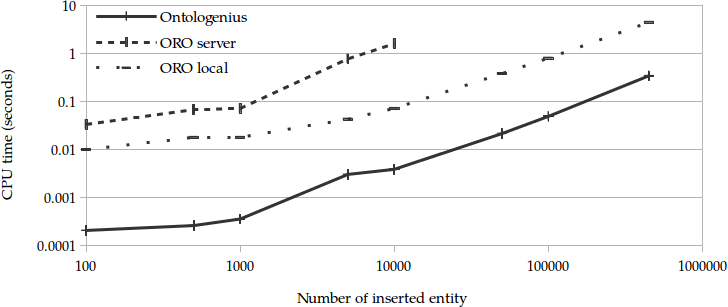
\includegraphics[width=\textwidth]{figures/chapter2/oro/R1.png}
\caption{\label{fig:chap2_oro_r1}Comparison of the required CPU time for querying for all the entities being animal, after that N entity have been created. Ontologenius and ORO are used with their communication layer. To assess the impact of the communication layer on ORO performance, we also provide measures without the ORO communication layer (ORO local).}
\end{figure}

For the test, ORO has been queried through the \sparql{} query where Ontologenius has been queried through low-level queries. To provide results representing the way the software should be used, both have been queried through their respective API. This means that results include the communication times. However, to not fall in a comparison of the communication layers but rather of the software, we have also tested to query ORO without the communication layer. The three plots (one for Ontologenius with the communication layer and two for ORO one with the communication layer and one without) are presented in figure~\ref{fig:chap2_oro_r1}.

First of all, we can note that with the communication layer we have not achieved to go over 10,000 entity with ORO. Rather than a limitation of the software itself, here it is a limitation of the test which requires the retrieve of too many entities. Nevertheless, with ORO without the communication layer, we succeed to go to 450,000 entities. We can see that Ontologenius performs far better than ORO, even when ORO is tested without its communication layer. This means that even if the communication time impacts the results, it does not spoil them. In server usage, Ontologenius is more performant of a factor around 255 on average. In this test Ontologenius takes advantage of its reasoning process applied at the update, allowing a more direct search.

For the two next queries, we only present the results in server usage as we just saw that this additional time is not inordinate. The second query uses the inverse properties. It aims at retrieving all the entities being under the \textit{apple}. As for the previous query, we thus expect to retrieve the N newly created entities. The corresponding \sparql{} query is:

\begin{quote} 
\centering 
?i isUnder apple
\end{quote}

The third query is more complex and uses a conjunction. The query aims at retrieving all the entities having a relation involving the property \textit{isAt} toward an entity being of type \textit{Plant}. Since all the newly created entities have a relation using the property \textit{isOn}, which is a sub-property of \textit{isAt}, toward the entity \textit{apple}, which inherites of the \textit{Plant} class, the N individual are expected to be retrieve. The corresponding \sparql{} query is:

\begin{quote} 
\centering 
?i isAt ?p, ?p rdf:type Plant
\end{quote}

The results of these two queries are presented for both software in figures~\ref{fig:chap2_oro_r3} and~\ref{fig:chap2_oro_r2}. They are almost the same as those of the first test query. Ontologenius performs on average better of a factor around 250 and we previously saw that the ORO communication layer has a limited impact which cannot explain such difference.

\begin{figure}[ht!]
\centering
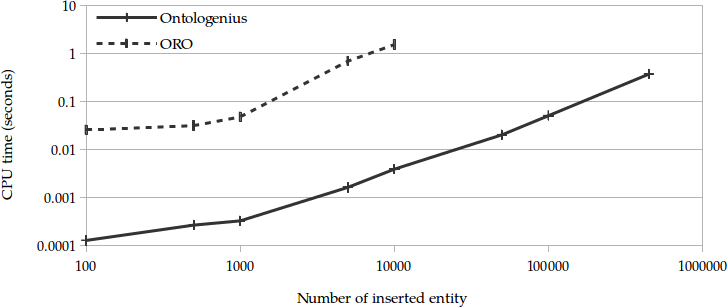
\includegraphics[width=\textwidth]{figures/chapter2/oro/R3.png}
\caption{\label{fig:chap2_oro_r3} Comparison of the required CPU time for querying all the entities having a relation of the kind ``isUnder'' toward a given entity. Since the invert relation has been inserted for all the created entity, the software has to solve the inverse relation to answer the query. Ontologenius and ORO are used with their communication layer.}
\end{figure}

\begin{figure}[ht!]
\centering
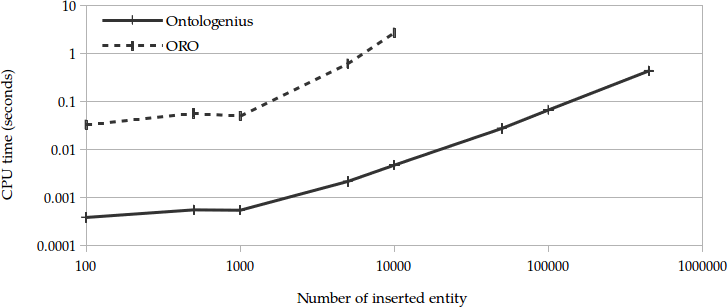
\includegraphics[width=\textwidth]{figures/chapter2/oro/R2.png}
\caption{\label{fig:chap2_oro_r2} Comparison of the required CPU time for querying all the entities having a relation of the kind ``isAt'' toward an entity of type ``Plant''. Ontologenius and ORO are used with their communication layer.}
\end{figure}

Through the comparison with ORO, considering its expected usage, we can fairly conclude that Ontologenius seems to be more adapted for performance requirement. Nevertheless, the test itself could be discussed. The fact that the software has to retrieve such an amount of entities does not represent real use-cases. Moreover, in the light of such equivalent results from a query to another, we can questionned what is really measured here. Looking backwards to the tests with KnowRob, the query time of Ontologenius was quite constant where here we have a constant increase. This test is however complementary with the ones of KnowRob, showing Ontologenius ability to retrieve a large number of entities. In addition, even with few entities (100), the performance gap is already significant, confirming the usability of Ontologenius even if it is not based on any established libraries like Jena or Pellet. 

\subsection{Additional tests}

With the previous tests, we have performed comparisons based on tests proposed by others contributions. We now present some additional tests to assess the performance of Ontologenius. Among the number of features, we have selected two of them.

We first propose to compare the required CPU time to retrieve an entity by its name in natural language and its identifier. For this test, we have taken 466,508 English words. These words have a length going from 1 letter to 45 letters with a means of  9.42 words. For each step of the test, N words have been randomly selected and inserted in the ontology as individuals. In addition, to each entity, we have defined a name in natural language, which is the same as the identifier. The N inserted entities have then been retrieved with their name in natural language and their identifier. The results are presented in figure~\ref{fig:chap2_extra_find}. The retrieve of an entity through the use of its identifier is constant with a required CPU time of around 0.046ms. At the difference, retrieving an entity through the use of its name in natural language is highly impacted by the size of the \acrshort{kb}. We reach a CPU time of 0.62ms for a \acrshort{kb} with 450,000 entity. This result highlights the fact that the name in natural language should be used, with Ontologenius, as an interface with the human partner and that all the algorithm should rather use the identifier. Even if this result could seem evident, it still shows the constant CPU time with the use of identifier, and that, even with large \acrshort{kb}.

\begin{figure}[ht!]
\centering
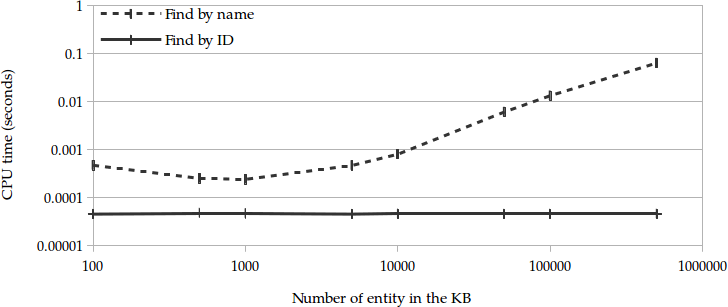
\includegraphics[width=\textwidth]{figures/chapter2/extra_tests/find.png}
\caption{\label{fig:chap2_extra_find} Comparison of the required CPU time to retrieve an entity by its name in natural language and its identifier. Ontologenius is used with its communication layer for both cases.}
\end{figure}

The second feature of Ontologenius we choose to evaluate is the instance copy. As explained earlier in this chapter, with Ontologenius we are able to make a deep copy of an ontology instance, resulting in a new and independent instance. Moreover, we have presented a kind of versioning mechanism allowing to represent multiple knowledge state in a single instance. We explained that the expected usage is to perform a single copy to create an independent instance, not altered by other components, then to use the versioning mechanism on the newly created instance. The presented test aims a measuring the required CPU time to perform such a copy, depending on the ontology size.

\begin{figure}[ht!]
\centering
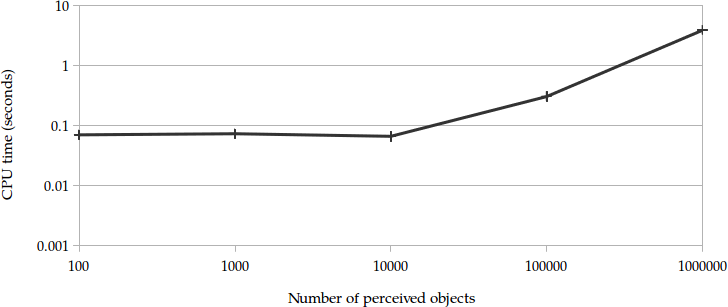
\includegraphics[width=\textwidth]{figures/chapter2/extra_tests/deepcopy.png}
\caption{\label{fig:chap2_extra_deepcopy} Evaluation of the required CPU time to perform a deep-copy depending on the number of perceived entity, represented in the Knowledge Base. Ontologenius is used with its communication layer. }
\end{figure}

For this test, we have taken again, the ontology content proposed by the KnowRob tests. It consists of inserting visual perception structures. We thus add N structures resulting in the creation of 2*N entities, 2*N raw data, 2*N inheritance links, and 3*N relations. Once the N structure inserted, we performed an instance copy and measured the required CPU time. The results for N going from 100 to 1,000,000 are represented in figure~\ref{fig:chap2_extra_deepcopy}. As expected, the required CPU time grows with the \acrshort{kb} size. Starting around 100ms for the smallest \acrshort{kb}, it grews to 4s for the largest one. Even if the results seem acceptable regarding the job to perform, we can however conclude that such an operation should not be performed too frequently. This reinforces the idea of doing a single copy then using the versioning mechanism if we want to represent many states of the same \acrshort{kb}.
